% % % % % % % % % % % % % % % % % % % % % % % % % % % % % % % % % % % % % % % % %
% INTRO
% % % % % % % % % % % % % % % % % % % % % % % % % % % % % % % % % % % % % % % % %
\section{Time box 7}
\listoftodos
\subsection{Time box planning}

\begin{figure}[H]
	\begin{centering}
		\missingfigure{Updated timebox figure}
		%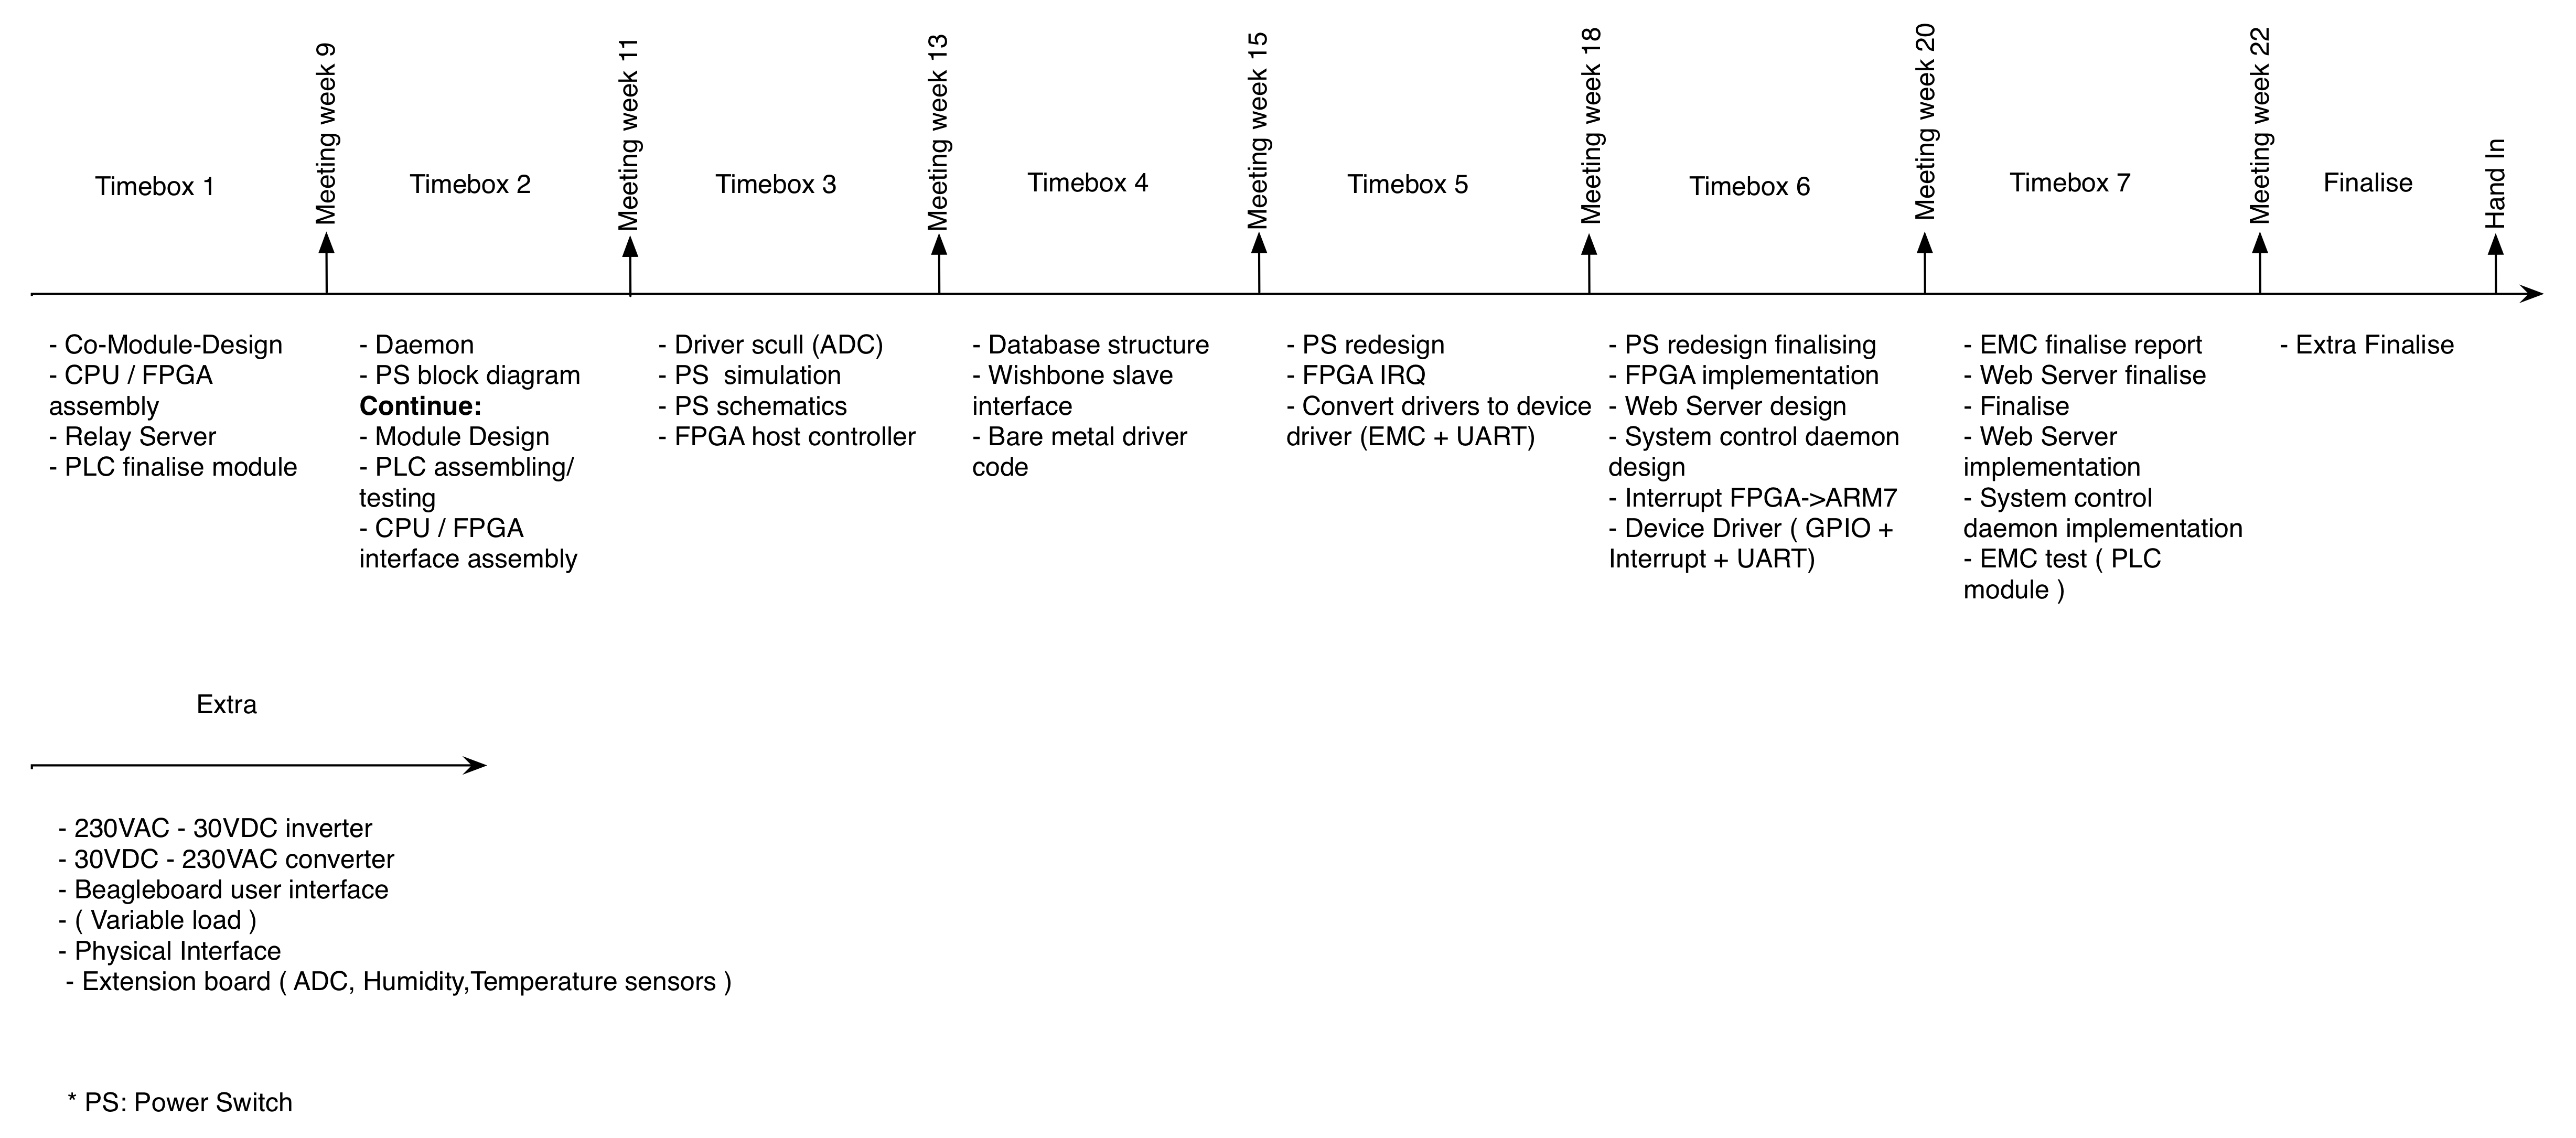
\includegraphics[width=1.0\textwidth]{images/tb_r5.png}
		%\caption{Updated time-box}
	\end{centering}
\end{figure}

\subsubsection{Work to be done in this time box}
\todo[inline]{Update List}
\begin{itemize}
	\item Requirements for debouncing
	\begin{itemize}
		\item Stability of switches
		\item Time limits
	\end{itemize}
	\item Verification
	\begin{itemize}
		\item External memory controller
		\item Verification of the Spartan 6
	\end{itemize}
	\item Jesus thing
		\begin{itemize}
			\item sub thing
		\end{itemize}
	\item Dennis thing
	\begin{itemize}
		\item Sub thing
	\end{itemize}
\end{itemize}

\paragraph{Description:}
\todo[inline]{Update Description}
\begin{description}
	\item[Requirements for debouncing] This is the timing requirements for the switch block to avoid bouncing when switching state
	\item[Verification] This is verification of the VHDL design including the EMC part in the LPC2478
	\item[Jesus thing]
	\item[Dennis thing]
\end{description}

\subsubsection{Time planning}

\begin{table}[H]
\centering
	\todo[inline]{Update Time}
	\begin{tabular}{|l|c|c|c|c|c|}
		\hline
		~			& Requirements for debouncing	& Verification			& Jesus thing		& Dennis thing	\\ \hline
		Estimation	& 3								& 7						& xx				& xx			\\
		Actual		& 3 							& xx					& xx				& xx			\\
		Developer	& Theis							& Theis					& Paulo				& Dennis		\\
		\hline
	\end{tabular}
	\caption{Estimation and actual time used on the project}
\end{table}
% % % % % % % % % % % % % % % % % % % % % % % % % % % % % % % % % % % % % % % % %
% % % % % % % % % % % % % % % % % % % % % % % % % % % % % % % % % % % % % % % % %
% Theis Thing
% % % % % % % % % % % % % % % % % % % % % % % % % % % % % % % % % % % % % % % % %
\subsection{Requirements for debouncing - Theis}
%			Intro
%					verification specification
%					deployment specification
%
This section is requirement update for the Switch block from section \ref{sec:Switch interrupt}.
\subsubsection{Analysis}
%			Analysis
%
%                Refactored block diagram
%                Refactored class diagram
%                Detailed use cases
%                User interface specification
%                System interface specification
%                Dimensioning specification 
%
In order to figure out how long the switches is bouncing, some measurement has been made on the switches, while it is shifted. The result is shown below.
\begin{figure}[H]
	\begin{centering}
		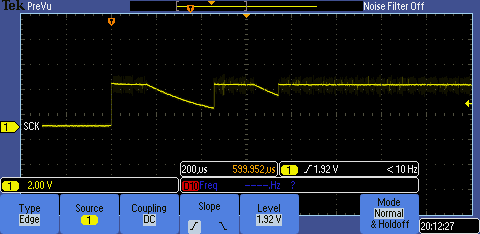
\includegraphics[width=0.7\textwidth]{images/debon_LtoH.png}
		\caption{Signal from switch. Low to high}
	\end{centering}
\end{figure}
From the figure above it is clear that the switch is bouncing, and it is possible to see how long it takes the switch to be stable. From the measurements it takes around $750\mu s$.
\begin{figure}[H]
	\begin{centering}
		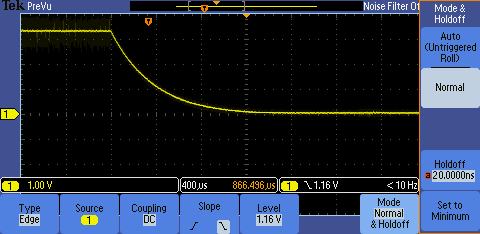
\includegraphics[width=0.7\textwidth]{images/debon_HtoL.png}
		\caption{Signal from switch. High to low}
	\end{centering}
\end{figure}
The figure above shows the switch signal from high to low, this signal is now bouncing, and would not cause any problem because the slope is negative at all time, so when the signal hits the point where the Spartan 6 is switching, the signal would not trigger a switch back. But is takes around $1200\mu s$ for the switch to stabilise.
\subsubsection{Design}
%       	 Design
%
%                UML/SysML deployment view(s)
%                Mechanical specifications and dimensioning
%                HW module specification per block
%                UML SW deployment view
%                Class specification
%                Refactored class diagram
%                Use case scenarios specifications
%                Sequence diagrams
%
In order to remove any debouncing on the switches, a delay is needed. In this system the time has to be the double plus one bit. From the measurements the longest time is $1200\mu s$, the double of that is $2400\mu s$. Calculations for the delay is shown below.
\begin{align}
	t &=	1200\mu s \cdot 2 \\
	f &=	100MHz\\
	t &=	2^{n}\cdot \dfrac{1}{f}\\
	n &=	\dfrac{\ln(f\cdot t)}{\ln(2)}\\
	n &=	\dfrac{\ln(100MHz\cdot 2400\mu s)}{\ln(2)}\\
	n &=	17.87
\end{align}
The bit length for the double delay is 18 and plus 1 bit, a 19 bit vector has to be used in the delay. The delay for 19 bit vector is.
\begin{align}
	t &=	2^{19}\cdot \dfrac{1}{100MHz}\\
	t &=	5.243 ms\\
\end{align}
This is the time delay that is used to debounce the switches.
\subsubsection{Conclusion}
This time delay has been tested in timebox 6 and it is working with the interrupt register in the Spartan 6.
%
%
%
% % % % % % % % % % % % % % % % % % % % % % % % % % % % % % % % % % % % % % % % %
\subsection{Verification - Theis}
%			Intro
%					verification specification
%					deployment specification
%
From the former timeboxes the blocks in the Spartan 6 has been implemented to make a complete system, which is communicating with the external memory controller in the LPC2478.
\subsubsection{External memory controller}
The EMC interface has been analysed with timings and signal assignment in order to make the Spartan 6 read and write data on the right time. On the figure below a block diagram for the EMC in the LPC2478 is shown. The data and pictures is taken from the \textit{LPC24xx user manual}\footnote{\url{http://www.nxp.com/documents/user\_manual/UM10237.pdf}} and the \textit{electrical datasheet}\footnote{\url{http://www.nxp.com/documents/data\_sheet/LPC2478.pdf}} for the LPC2478
\begin{figure}[H]
	\begin{centering}
		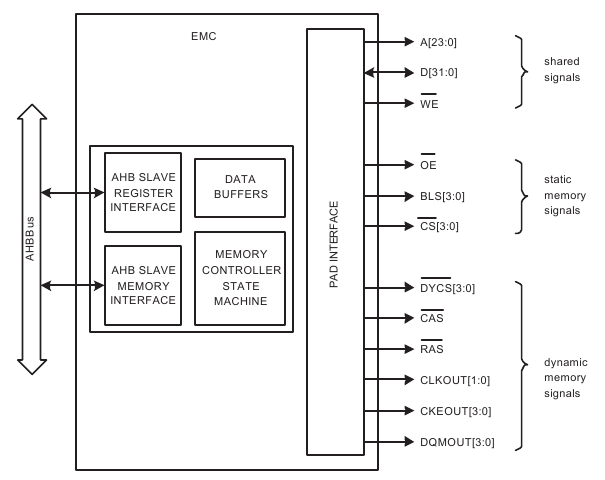
\includegraphics[width=0.8\textwidth]{images/tb7_EMC_block.png}
		\caption{EMC block}
	\end{centering}
\end{figure}
The EMC is used in static mode without the \textit{BLS}\footnote{Byte lane selects} signal, and for memory selection it is only using the \textit{CS2}\footnote{Chip Select 2} for the Spartan 6, this is the interface that has to be implemented in the Spartan 6 to control the wishbone master. The block that takes care of this assignment is the host controller from timebox 3. The timings and signal assignment is shown on the next to figures.
\begin{figure}[H]
	\begin{centering}
		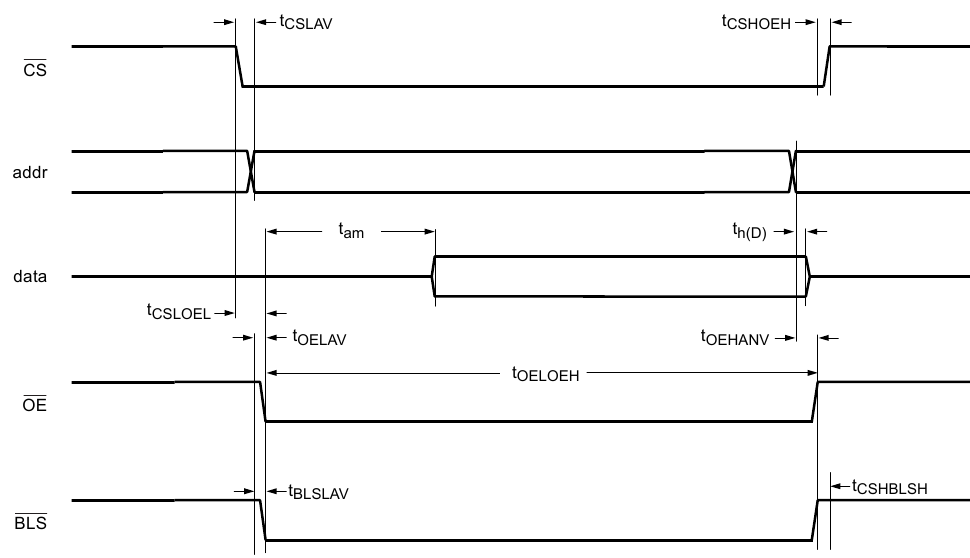
\includegraphics[width=0.8\textwidth]{images/tb7_EMC_read.png}
		\caption{EMC Read timing}
	\end{centering}
\end{figure}
The important thing when the EMC read data from the Spartan 6, is the $t_{am}$ this is where the EMC reads the data from the Spartan 6, therefore the Spartan 6 has to have valid data ready latest at that time, for the EMC to read correct data. From the electrical datasheet the timing for $t_{am}$ is taken.
\begin{align}
t_{am}min &= (WAITRD - WAITOEN + 1) \cdot T_{cy} - 12.70ns\\
t_{am}typ &= (WAITRD - WAITOEN + 1) \cdot T_{cy} - 9.57ns\\
t_{am}max &= (WAITRD - WAITOEN + 1) \cdot T_{cy} - 8.11ns
\end{align}
The \textit{WAITRD} and \textit{WAITOEN} is integer values that is set in the setup of the EMC in the LPC2478, \textit{WAITRD} has influence on the timing of $t_{am}$ and \textit{OELOEH} increasing this value increase the timing. When \textit{WAITOEN} is increased \textit{CSLOEL} is increased to and $t_{am}$ and \textit{OELOEH} is decreased. The $T_{cy}$ is the time of the clock period.
\begin{align}
CCLK &= 72MHz\\
T_{cy} &= \dfrac{1}{CCLK}\\
T_{cy} &= 13.889ns
\end{align}
The exact timing of $t_{am}$ is calculated late with the Bus functional module used for verification of the Spartan 6 design.
\begin{figure}[H]
	\begin{centering}
		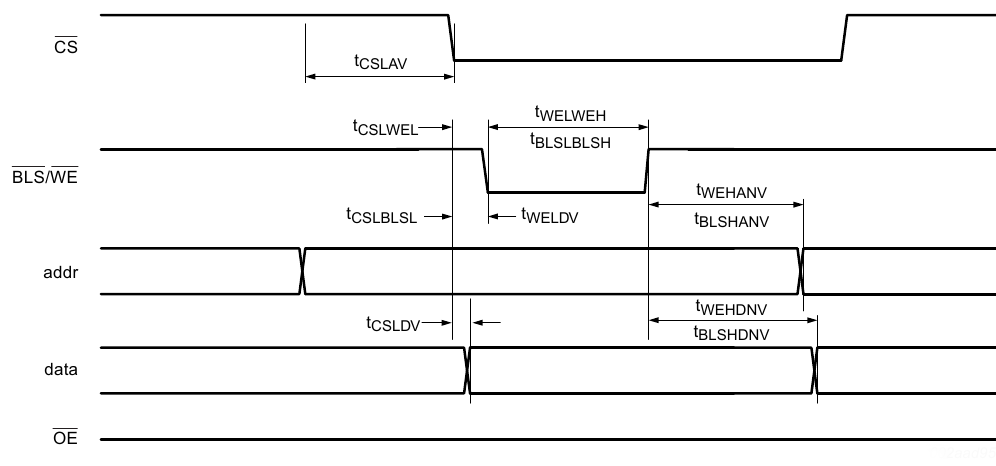
\includegraphics[width=0.8\textwidth]{images/tb7_EMC_write.png}
		\caption{EMC Write timing}
	\end{centering}
\end{figure}
The write diagram shows that the data is valid at the same time as \textit{WE}\footnote{Write Enable} is set low, as long as the Spartan 6 is reacting on \textit{CS2} and the \textit{WE} invalid data is not a problem.
\subsubsection{Bus functional module}
The bus functional module is a module written in VHDL for test purpose. A BFM is able to simulate different interfaces, depending on the code. In this project the BFM is used to test the total design of the Spartan 6 by simulating the EMC interface from the LPC2478. A rough code sketch was handed out from Morten Opprud Jakobsen, timing tweaks needed to be updated in order to make a correct simulation.\\
\dirtree{%
.1 \textcolor{blue}{sim}. 
.2 arm\_emc\_package.vhd. 
.2 \textcolor{blue}{log}. 
.3 arm7\_bfm\_log.txt. 
.2 \textcolor{blue}{stim}. 
.3 arm7\_bfm\_stim.dat. 
.2 tb\_ARM\_BFM.vhd. 
.2 txt\_util.vhd\\. 
}
The file structure of the BFM is shown above, in \textit{arm\_emc\_package.vhd} all the timings and constants is contained. This file also holds the functions for a read and write cycle, with signal assignment in the correct order and time from the timings. \textit{txt\_util.vhd} holds function for converting text strings. The \textit{tb\_ARM\_BFM.vhd} is the test bench file, this file takes a data input from the data file. The data file tells the BFM what to do, if it shall read, write, wait or log something, the logs is written to the log file. The BFM is used on the final Spartan 6 design with the following data file.
\begin{lstlisting}[caption=BFM data file]
#WAIT 10
#LOG Write 0x00 to LEDs
#WR 0000000000010000 0000000000000000
#LOG Change switches
#SW 01000000
#WAIT 30
#LOG Read IRQ reg
#RD 0000000000000000
#LOG Read switch reg
#RD 0000000000100000
#LOG Write 0x00 to LEDs
#WR 0000000000010000 0000000001000000
#WAIT 10
#END
\end{lstlisting}
The test bench signals is shown below. In the first figure, the BFM write to the LEDs to turn off, in the figure it is shown that the LEDs is changed to all zeros. Next the switches positions is changed, the arrow shows that the interrupt to the LPC2478 is activated after the switches is changed.
\begin{figure}[H]
	\begin{centering}
		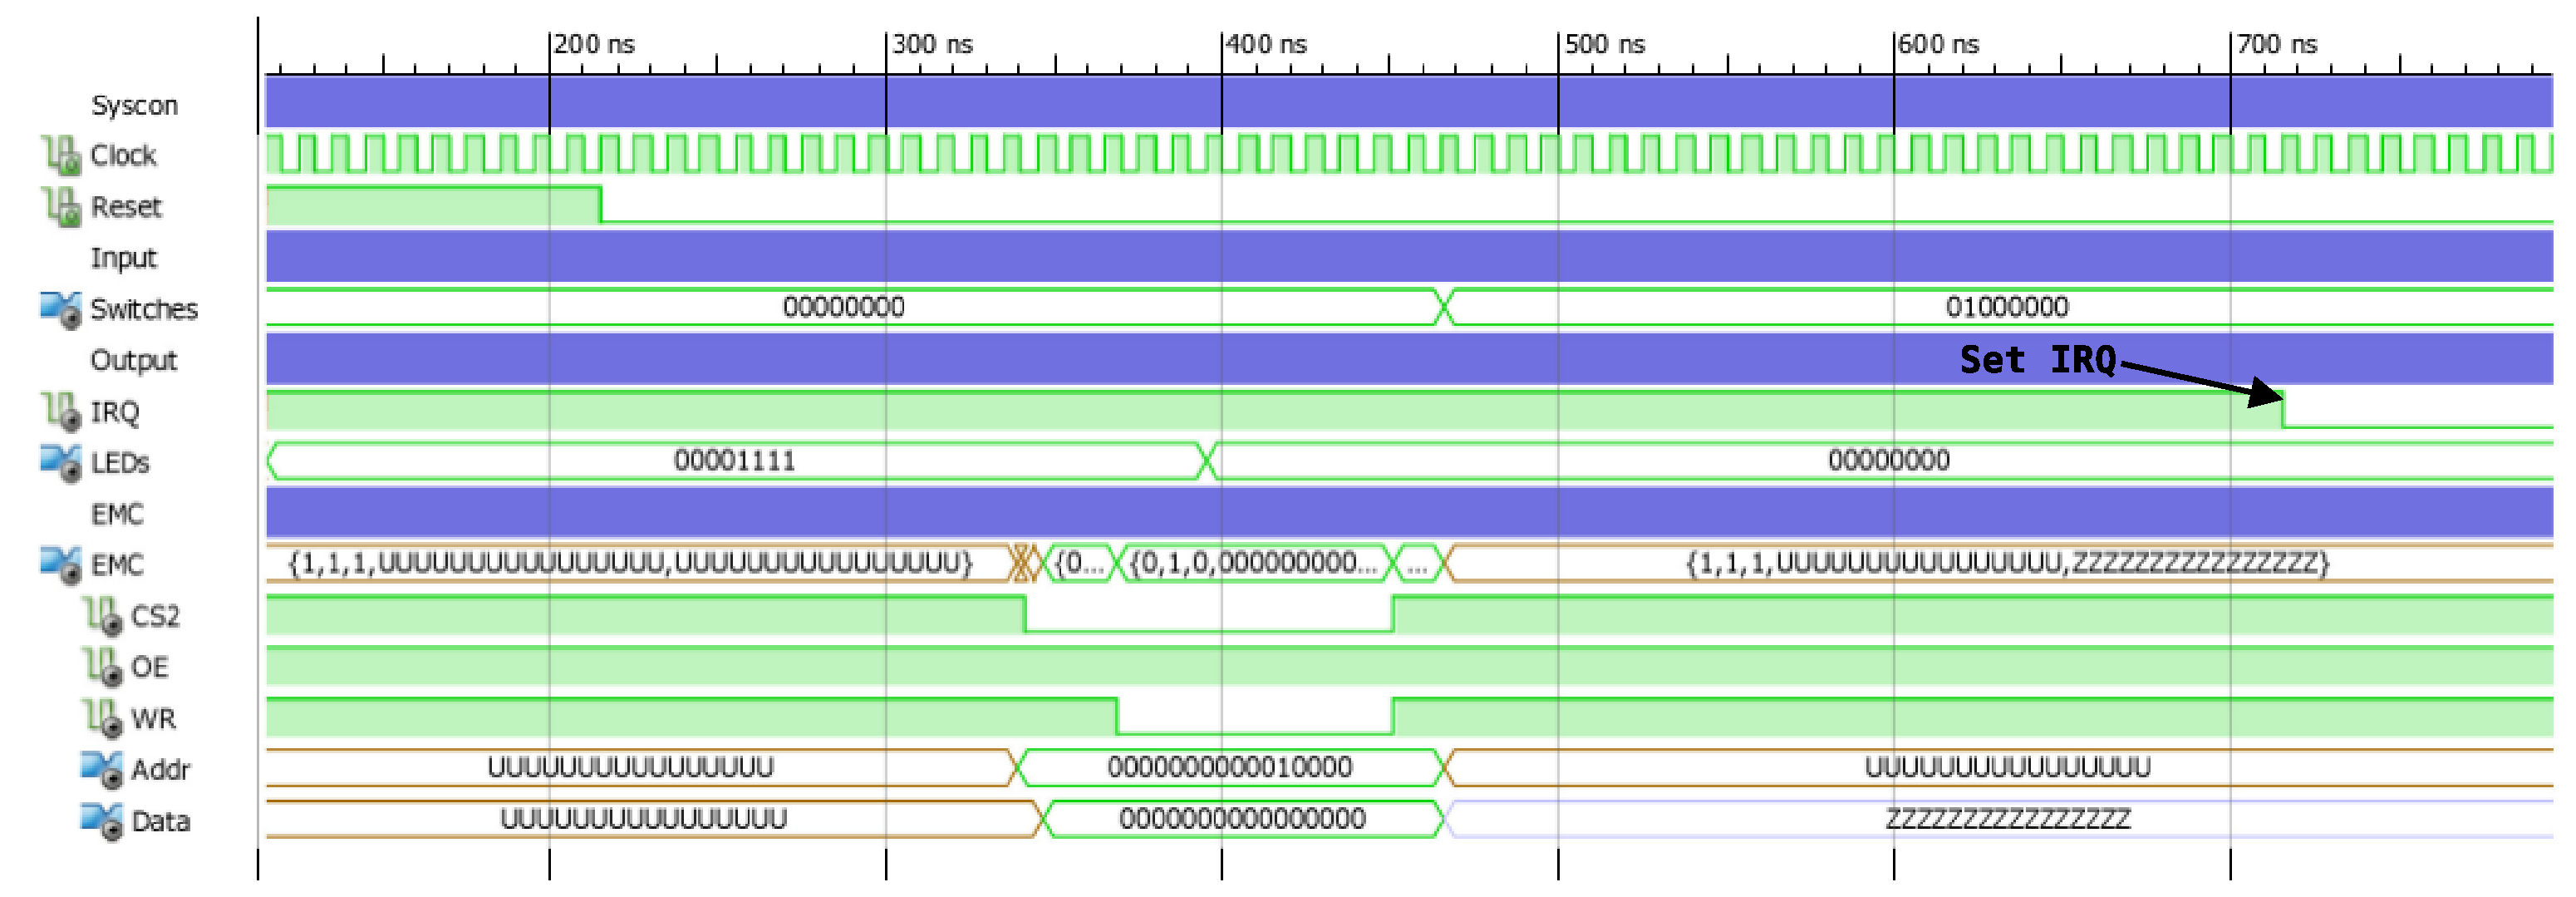
\includegraphics[width=1.0\textwidth]{images/tb7_BFM_write.eps}
		\caption{BFM write}
	\end{centering}
\end{figure}
The figure below is the continued BFM test bench. First the BFM reads the interrupt register, the first arrow shows when the data is valid on the Spartan 6, the blue maker indicate when the EMC is reading data from the Spartan 6. The second arrow shows that the interrupt is deactivated as the interrupt register is read. Next the BFM read the switch register to get the switch position, the arrow again shows when the data is valid, and the blue marker show when the data is read. Last the LEDs is set to the new switch position by another write to the LEDs from the BFM.
\begin{figure}[H]
	\begin{centering}
		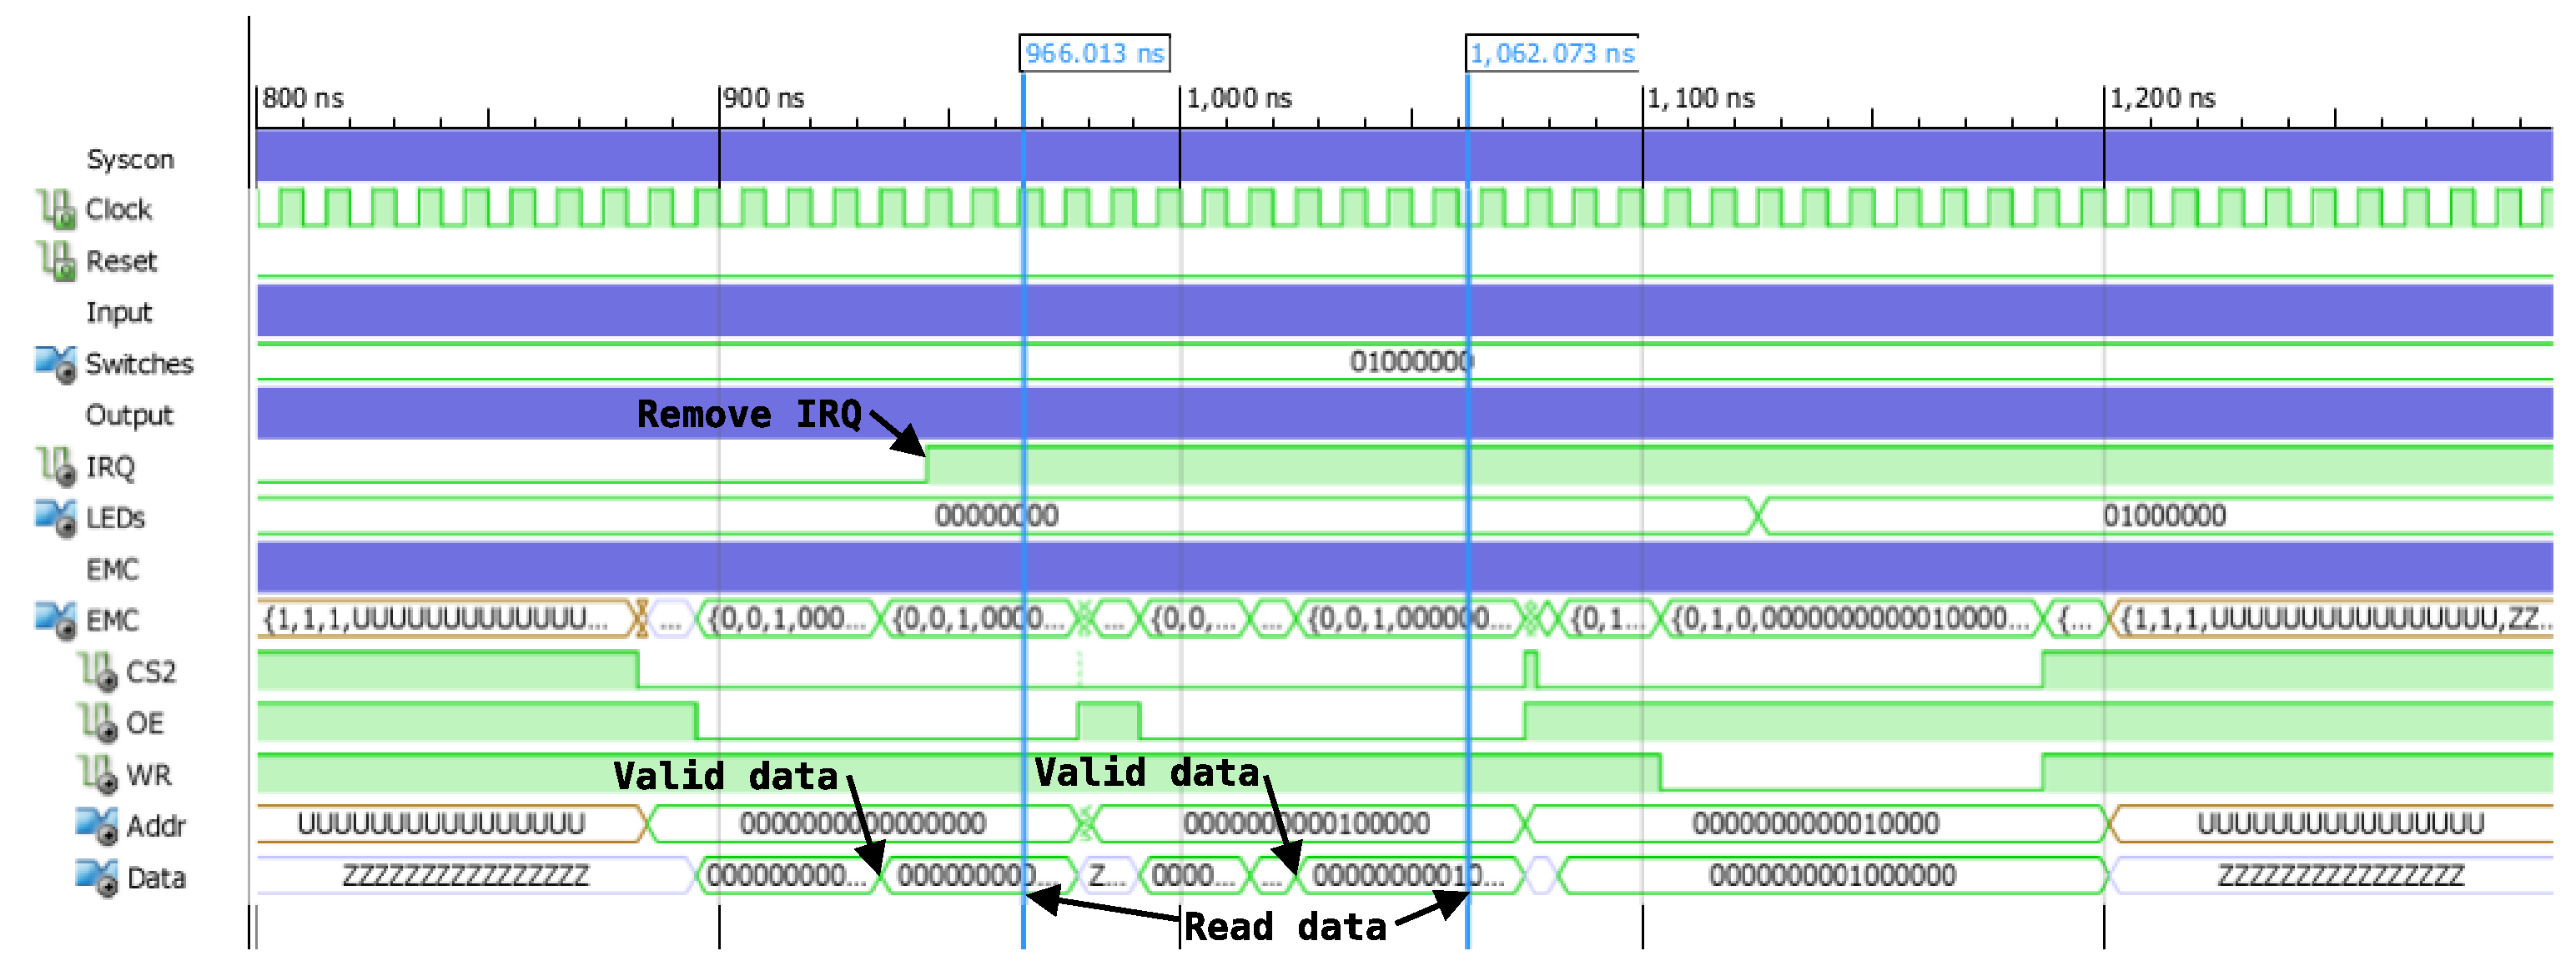
\includegraphics[width=1.0\textwidth]{images/tb7_BFM_read_irq.eps}
		\caption{BFM read IRQ}
	\end{centering}
\end{figure}
\subsubsection{Digital clock manager}
In the code handed out by Morten Opprud Jakobsen, there is a DCM\footnote{Digital Clock Manager}. The main purpose of this block is to multiply the $16MHz$ on Spartan 3 with a factor of 4 to get a $64MHz$ clock. In the Spartan 6 the normal clock speed is $100MHz$, so the multiplication is not necessary in this case. But it turns out that the EMC is not able to read or write any data on the Spartan 6 with use only of the standard clock. The reason for this could be \textit{jitter} on the clock. The DCM in Spartan 6 tolerates two types of jitter, \textit{cycle-to-cycle jitter} and \textit{period jitter}. Cycle-to-cycle jitter is the change in clock period from cycle to cycle, the period jitter is the change over millions of clock cycles. The code for the DCM is shown below.
\begin{lstlisting}[language=VHDL, caption=DCM\_SP]
...
	clk_o <= clk_r;

-- DCM instantiation for the system clock.
	DCM_Sys : DCM_SP
	generic map (
		CLKFX_DIVIDE				=> 2,											-- Can be any integer from 1 to 32
		CLKFX_MULTIPLY			=> 2)											-- Can be any integer from 2 to 32
	port map	(
				CLK0				=> clk_s,											-- 0 degree DCM CLK ouptput
				CLKFX				=> clk_r,											-- DCM CLK synthesis out (M/D)
				CLKFB				=> clk_s,											-- DCM clock feedback
				CLKIN				=> clk_i,											-- Clock input (from IBUFG, BUFG or DCM)
				RST					=> '0'												-- DCM asynchronous reset input
				);
...
\end{lstlisting}
It is not possible to multiply with one, so in order to not change the clock speed, the clock is multiplied with 2 and divided with 2. The DCM in the Spartan 6 has a lots of features, one feature that is not used in the project is to make phase shift in the clock, the feature that is used is removing the jitter, this is done in the code above. The DCM takes the standard clock input, and the zero phase shifted clock is routed into the clock feedback, for the DCM to compensate for jitter.
\subsubsection{Spartan 6}
The final design of the Spartan 6 in this project has been verified and the figure below shows the top layer block, and the inputs and outputs on the Spartan 6.
\begin{figure}[H]
	\begin{centering}
		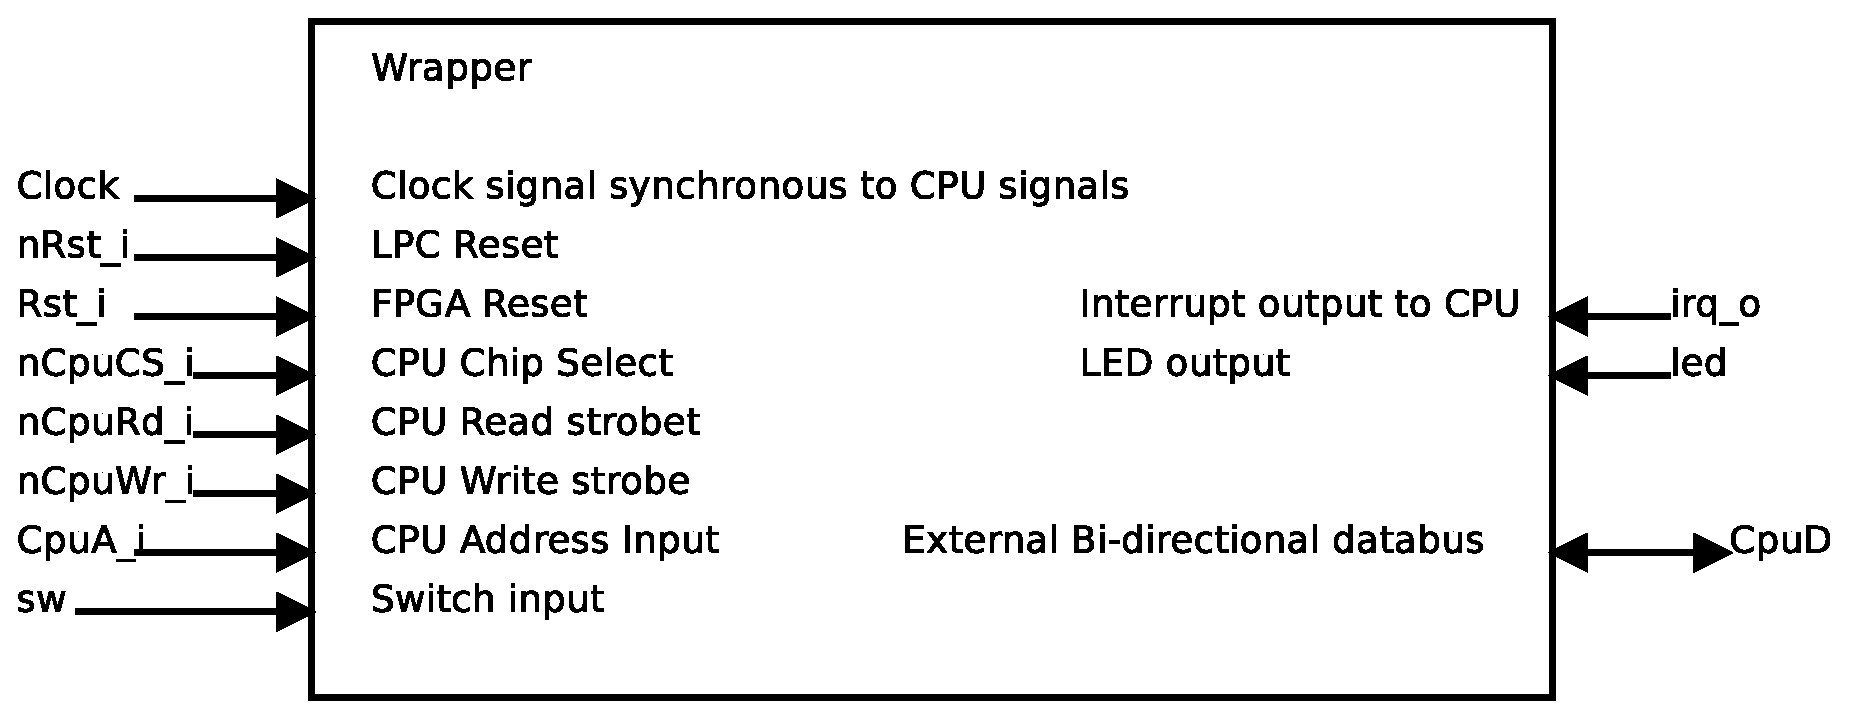
\includegraphics[width=0.9\textwidth]{images/tb7_wrapperblock.eps}
		\caption{Top level in Spartan 6}
	\end{centering}
\end{figure}
The Spartan 6 acts as a memory block seen from the EMC in the LPC2478, the memory map for the Spartan 6 is shown below, with slave addresses, data direction and data length.
\begin{table}[H]
    \begin{tabular}{|l|l|l|l|l|l|p{3.7cm}|}
        \hline
        Name         & DIR		 & S select 	& S address 	& Data                & EMC address & Note                                  \\ \hline
        IRQ Register & Read      & 000          & 0000          & 7 bit - 6 down to 0 & 0x82000000        & Hold data from the interrupting slave \\ \hline
        LED          & Write     & 001          & 0000          & 8 bit - 7 down to 0 & 0x82000020        & Set states of LEDs                    \\ \hline
        Switch       & Read      & 010          & 0000          & 8 bit - 7 down to 0 & 0x82000040        & Hold state of switches                \\
        \hline
    \end{tabular}
    \caption{Memory map of Spartan 6\\
    		 S = Slave, DIR = Direction}
\end{table}
\subsubsection{Conclusion}
The BFM verify the design, and it has been tested on the hardware and it is working properly. It is not possible to measure the clock speed with the equipment at the university, so it is not possible to verify that the code fails without the DCM because of jitter on the clock.
% % % % % % % % % % % % % % % % % % % % % % % % % % % % % % % % % % % % % % % % %
% % % % % % % % % % % % % % % % % % % % % % % % % % % % % % % % % % % % % % % % %
% Jesus Thing
% % % % % % % % % % % % % % % % % % % % % % % % % % % % % % % % % % % % % % % % %
\subsection{Jesus thing - Paulo}
%			Intro
%					verification specification
%					deployment specification
%
\subsubsection{Analysis}
%			Analysis
%
%                Refactored block diagram
%                Refactored class diagram
%                Detailed use cases
%                User interface specification
%                System interface specification
%                Dimensioning specification 
%
\subsubsection{Design}
%       	 Design
%
%                UML/SysML deployment view(s)
%                Mechanical specifications and dimensioning
%                HW module specification per block
%                UML SW deployment view
%                Class specification
%                Refactored class diagram
%                Use case scenarios specifications
%                Sequence diagrams
%
\subsubsection{Implementation}
%     	   Implementation
%
%                Mechanical drawings with details explained
%                Electronic diagrams with details explained
%                Source code with details explained
%                Description of integration 
%
\subsubsection{Verification}
%       	 Verification
%
%                Module tests
%                Integration tests
%                Acceptance test
\subsubsection{Conclusion}
% % % % % % % % % % % % % % % % % % % % % % % % % % % % % % % % % % % % % % % % %
% % % % % % % % % % % % % % % % % % % % % % % % % % % % % % % % % % % % % % % % %
% Dennis Thing
% % % % % % % % % % % % % % % % % % % % % % % % % % % % % % % % % % % % % % % % %
\subsection{Dennis thing - Dennis}
%			Intro
%					verification specification
%					deployment specification
%
\subsubsection{Analysis}
%			Analysis
%
%                Refactored block diagram
%                Refactored class diagram
%                Detailed use cases
%                User interface specification
%                System interface specification
%                Dimensioning specification 
%
\subsubsection{Design}
%       	 Design
%
%                UML/SysML deployment view(s)
%                Mechanical specifications and dimensioning
%                HW module specification per block
%                UML SW deployment view
%                Class specification
%                Refactored class diagram
%                Use case scenarios specifications
%                Sequence diagrams
%
\subsubsection{Implementation}
%     	   Implementation
%
%                Mechanical drawings with details explained
%                Electronic diagrams with details explained
%                Source code with details explained
%                Description of integration 
%
\subsubsection{Verification}
%       	 Verification
%
%                Module tests
%                Integration tests
%                Acceptance test
\subsubsection{Conclusion}
% % % % % % % % % % % % % % % % % % % % % % % % % % % % % % % % % % % % % % % % %
% % % % % % % % % % % % % % % % % % % % % % % % % % % % % % % % % % % % % % % % %
% Deployment
% % % % % % % % % % % % % % % % % % % % % % % % % % % % % % % % % % % % % % % % %
\subsection{Deployment}
	%which versions of the prototype the customer will get
	%with what functionality.
\paragraph{Theis thing}
%
%
\paragraph{Jesus thing}
%
%
\paragraph{Dennis thing}
%
%